
%%%%%%%%%%%%%%%%%%%%%%% file typeinst.tex %%%%%%%%%%%%%%%%%%%%%%%%%
%
% This is the LaTeX source for the instructions to authors using
% the LaTeX document class 'llncs.cls' for contributions to
% the Lecture Notes in Computer Sciences series.
% http://www.springer.com/lncs       Springer Heidelberg 2006/05/04
%
% It may be used as a template for your own input - copy it
% to a new file with a new name and use it as the basis
% for your article.
%
% NB: the document class 'llncs' has its own and detailed documentation, see
% ftp://ftp.springer.de/data/pubftp/pub/tex/latex/llncs/latex2e/llncsdoc.pdf
%
%%%%%%%%%%%%%%%%%%%%%%%%%%%%%%%%%%%%%%%%%%%%%%%%%%%%%%%%%%%%%%%%%%%

\documentclass{llncs}
%\documentclass[runningheads]{llncs}

\usepackage{amssymb}
\setcounter{tocdepth}{3}
\usepackage{graphicx}
%\<andres> para que las graficas aparezcan dentro de la sección.
\usepackage[section]{placeins}
\usepackage{colortbl}
\usepackage{longtable}
% <maria> 

\usepackage{fancybox}
%\usepackage[T1]{fontenc}
\usepackage[ansinew]{inputenc}
%\usepackage{a4wide, url}
\usepackage{url}
\usepackage[normalem]{ulem}
%\newlength\wvtextpercent
%\setlength\wvtextpercent{0.009\textwidth}

\usepackage{verbatim}

\usepackage{array} % and/or

\newcommand{\keywords}[1]{\par\addvspace\baselineskip
\noindent\keywordname\enspace\ignorespaces#1}

\begin{document}

%\mainmatter  % start of an individual contribution

% first the title is needed
\title{vocab-express - Exploring the Vocabulary of a Dataset}

% a short form should be given in case it is too long for the running head
\titlerunning{vocab-express}

% the name(s) of the author(s) follow(s) next
%
% NB: Chinese authors should write their first names(s) in front of
% their surnames. This ensures that the names appear correctly in
% the running heads and the author index.
%
\author{Boris Villaz\'{o}n-Terrazas\inst{1}\and Michael Hausenblas\inst{2}}
%
%\authorrunning{Boris Villaz\'{o}n-Terrazas\and Michael Hausenblas}
% (feature abused for this document to repeat the title also on left hand pages)

% the affiliations are given next; don't give your e-mail address
% unless you accept that it will be published
\institute{OEG-DIA, FI, Universidad Polit\'ecnica de Madrid, Spain\\
\email{bvillazon@fi.upm.es}
\and
Digital Enterprise Research Centre, NUI Galway, Ireland\\
\email{michael.hausenblas@deri.ie}}


%\url{http://www.springer.com/lncs}}

%
% NB: a more complex sample for affiliations and the mapping to the
% corresponding authors can be found in the file "llncs.dem"
% (search for the string "\mainmatter" where a contribution starts).
% "llncs.dem" accompanies the document class "llncs.cls".
%

\maketitle
\begin{abstract}
One of the drawbacks of the reuse, review or query LOD datasets is the lack of mechanisms that provides an overview of the structure of them.
One step forward to have such overview of the structure is getting the vocabulary used by the datasets. In this paper we present a brief description of vocab-express that aims at exploring the vocabulary of a dataset.
\keywords{Linked Data, RDF Dataset, Vocabulary} 
\end{abstract}

\vspace{-2mm}
\section{Introduction and Motivation}\label{sec:introduction}
So far, Linked Data principles and practices are being adopted by an increasing number of data providers, getting as a result a global data space on the Web containing thousands of LOD datasets \cite{}. In order to reuse, review or query a dataset published on the Web of Data, it is important to know the structure of the data. One step forward for knowing in depth the structure of the data is to explore the vocabulary that the dataset is using, and how the dataset is using such vocabulary.

There are available works such as (1) \emph{LODStats} \cite{} that provides the information related with the vocabulary of given dataset, and (2) \emph{make-void} \cite{} that computes statistics about RDF files. However, LODStats is thought for the whole set of LOD datasets registered in The Data Hub \footnote{\footnotesize \url{http://thedatahub.com}}, and it is based on declarative descriptions of those datasets, and \emph{make-void} is thought for RDF files but not for RDF datasets.

In this paper we present vocab-express\footnote{\footnotesize \url{http://vocab-express.nodester.com/}}, a simple tool for exploring the vocabulary of a given dataset. The tool provides all the related information to the vocabulary of the dataset (1) list of all classes, (2) list of all the properties, (3) the number of instances of each class, (4) the number instances of each property, (5) the language of labels and comments, of the vocabulary elements.




\vspace{-2mm}
\section{vocab-express overview}\label{sec:vocab}
vocab-express is being implemented in node.js\footnote{\footnotesize \url{http://nodejs.org/}}, which is a platform built on V8\footnote{\footnotesize V8 is Google's open source JavaScript engine.} for easily building fast, scalable network applications. 
Figure \ref{fig:workflow} depicts the workflow of vocab-express. Next we describe the steps of the workflow

\begin{figure}[hbt!p]
\begin{center}
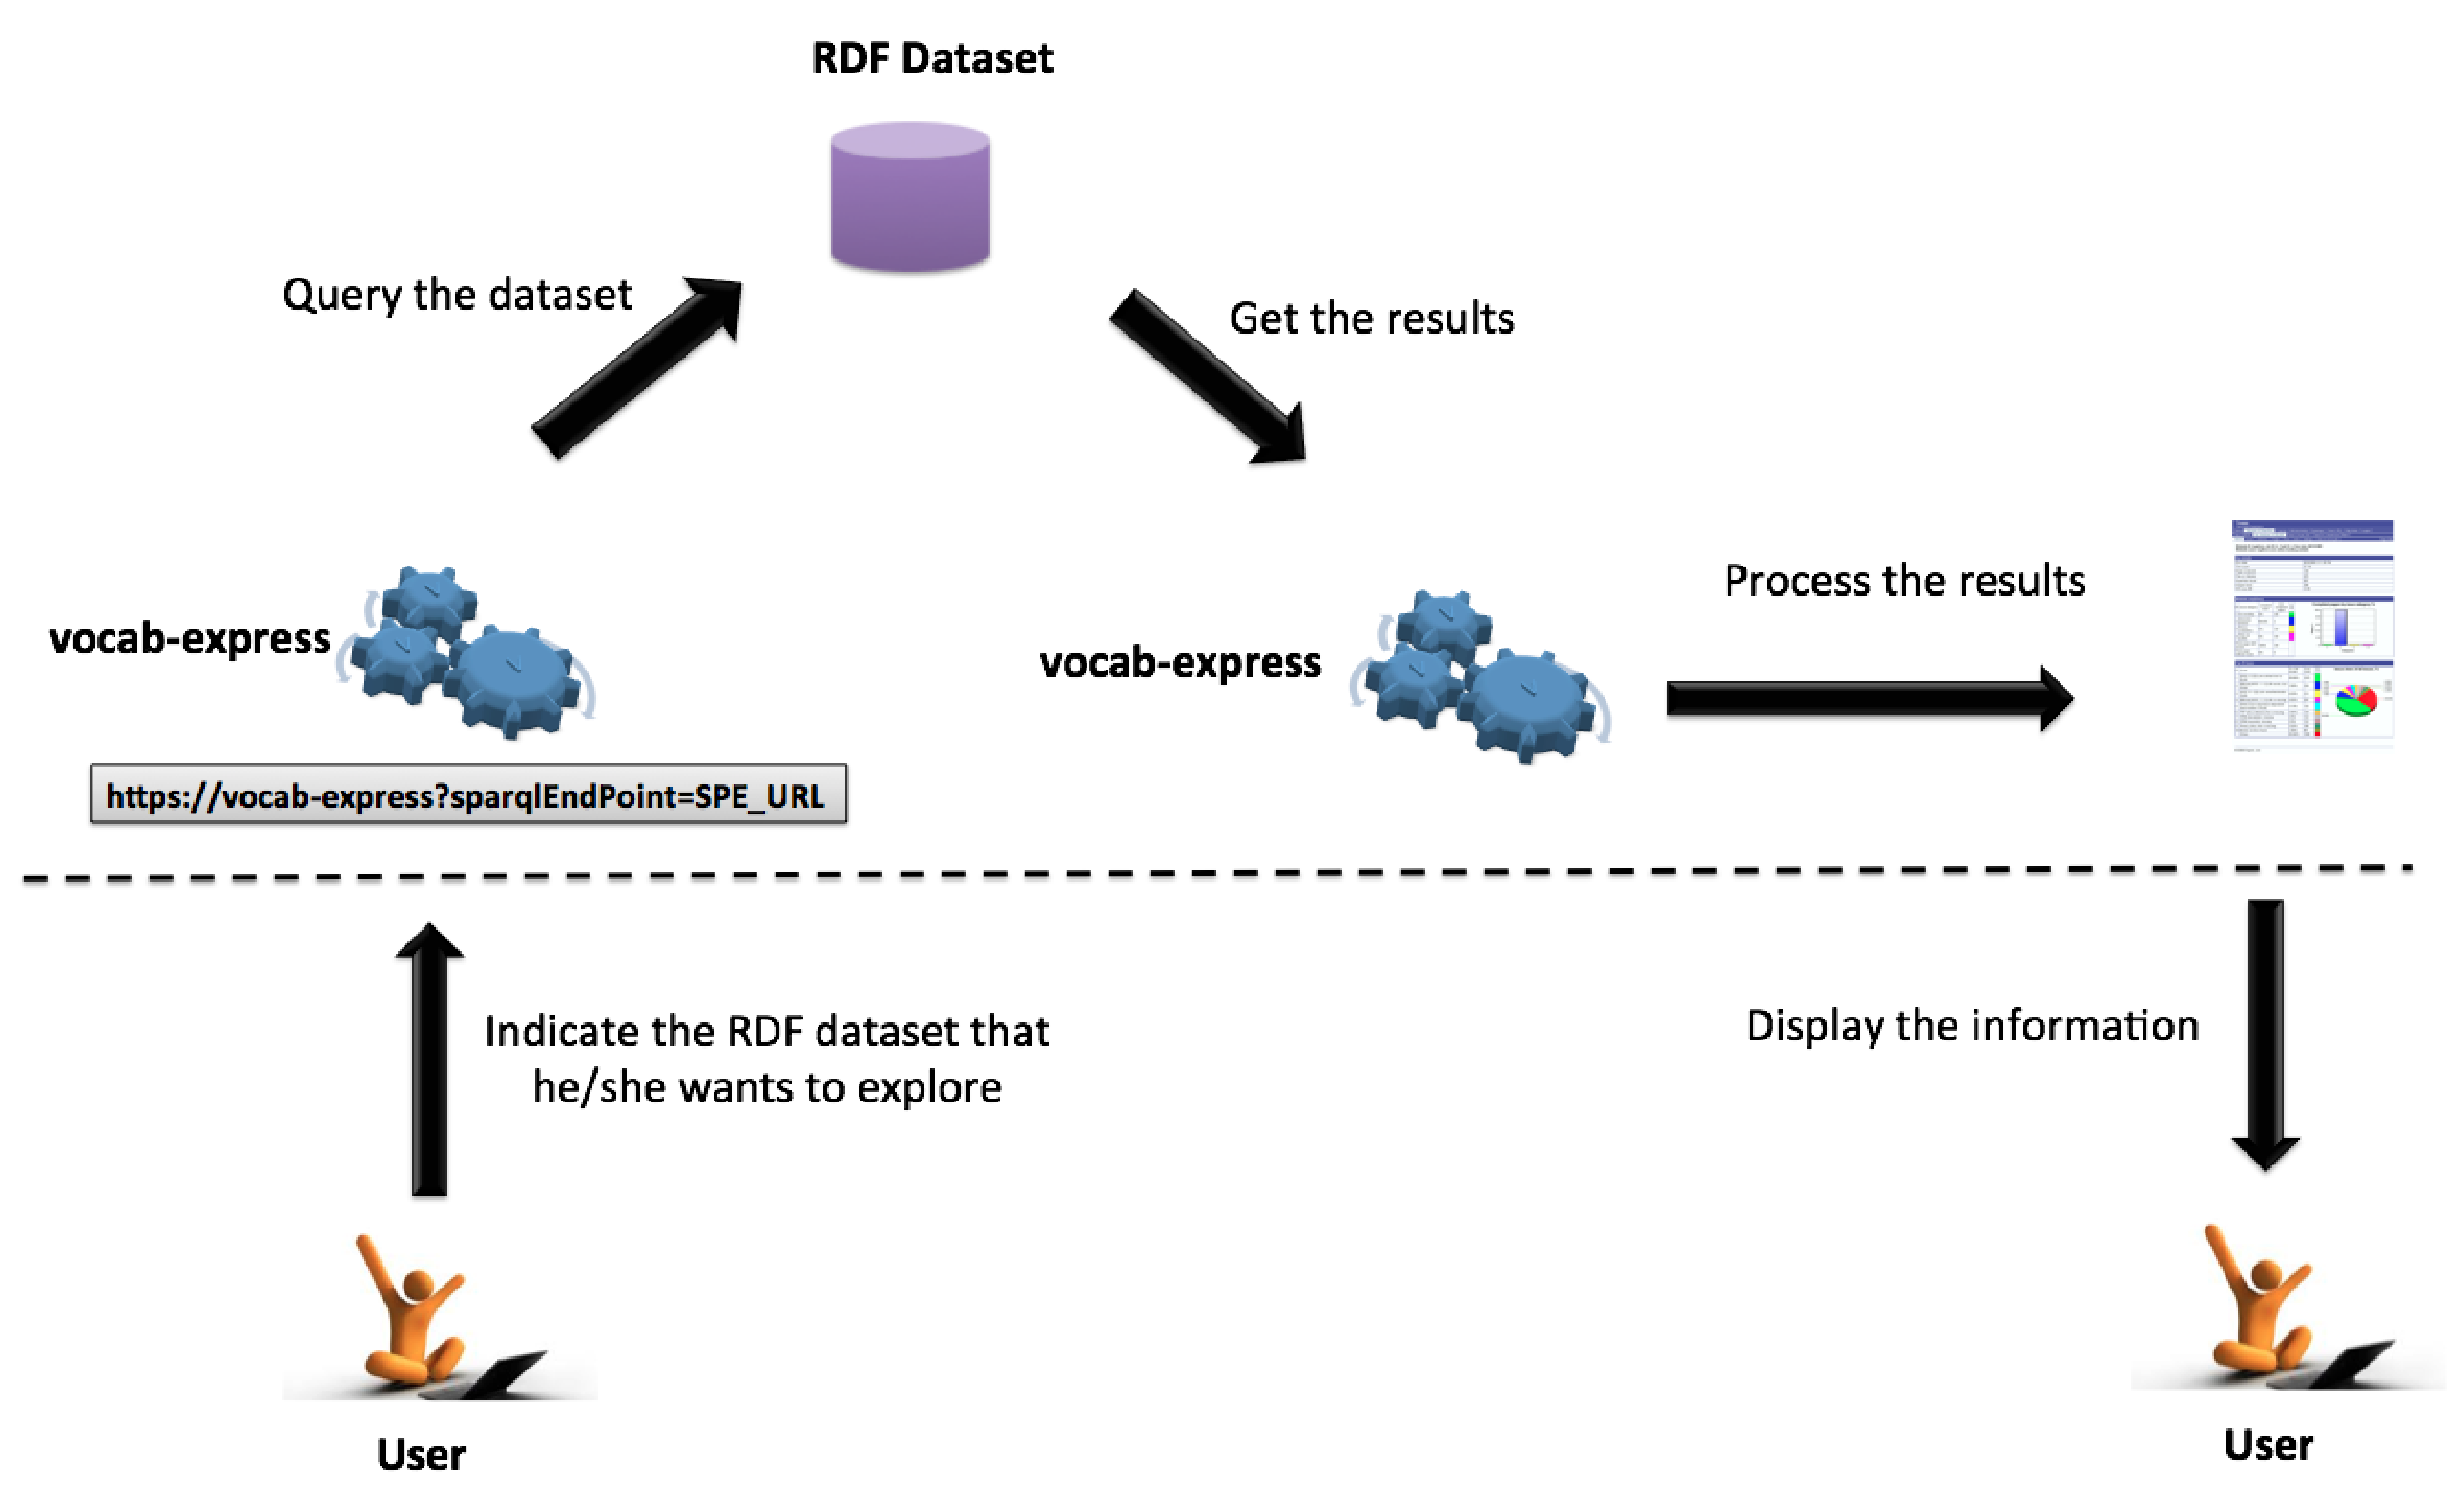
\includegraphics[scale=0.22]{img/workflow.eps}
\end{center}
\label{fig:workflow} 
\caption{vocab-express workflow}
\end{figure}


\begin{enumerate}
	\item The user indicates the RDF dataset he/she wants to explore by providing its SPARQL endpoint URL
	\item vocab-express receives and validates the SPARQL endpoint URL
	\item vocab-express queries the SPARQL endpoint and gets results in JSON\footnote{\footnotesize \url{http://www.json.org}} format
	\item vocab-express processes the results and displays the information to the user
\end{enumerate}
The workflow is similar if the user provides the URL of the VoID file instead of the SPARQL endpoint.

\vspace{-4mm}
\section{Conclusions}\label{sec:conclusions}
In this paper we have presented our ongoing work for exploring the vocabulary of an RDF dataset.


 
%\vspace{2mm}
%\textbf{Acknowledgments.}

\vspace{-2mm}
\bibliographystyle{abbrv} 
\bibliography{vocab-e} 



\end{document}
